\documentclass{mcmthesis}		    %使用mcm模板
\mcmsetup
{
	tcn = 2001334,				%你的team control number 队伍控制编号
	problem = B,				%你选的题号
	sheet = true, 				%是否要mcm摘要页
	titleinsheet = true, 		%是否在摘要页显示标题
	keywordsinsheet = true,		%是否把关键词放到摘要页
	titlepage = false, 			%是否要一个标题页
	abstract = true				%是否在摘要页显示摘要
}


% 常用命令
\def\ie{\mbox{\textit{i.e.}}}
\def\eg{\mbox{\textit{e.g.}}}
\def\wrt{\mbox{\textit{w.r.t. }}}
\DeclareMathOperator*{\argmin}{arg\,min}
\DeclareMathOperator*{\argmax}{arg\,max}

\usepackage{algorithm}
\usepackage{algorithmic}
\usepackage{palatino}				%字体
\usepackage{palatino}				%字体
\usepackage{geometry}				%边距
\usepackage{graphics}
\usepackage{subfigure}
\usepackage{amsmath}
\usepackage{siunitx}
\usepackage{indentfirst}
\usepackage{multirow}


\def\djy{\textcolor{black}}
\def\lyx{\textcolor{black}}
\def\gjx{\textcolor{black}}


 
\bibliographystyle{plain}

\graphicspath{{figure/}}%图片在目前目录下的figure下
% \geometry{left=1.93cm,right=1.93cm,top=1.9cm,bottom=2.40536cm} %页边距
\geometry{left=2.23cm,right=2.23cm,top=1.9cm,bottom=2.40536cm} %页边距
\linespread{1} 					%行间距
\setlength{\parskip}{0em} %%临时为摘要页设置一个比较小的段间距
% \setlength{\parindent}{1.5em}
\bibliographystyle{plain}
\title{\textbf{A Simulation System of Sandcastle Foundation Based On Cellular Automata}}			%修改标题

\hypersetup{colorlinks,linkcolor=black,anchorcolor=black,citecolor=black}
\begin{document}
	\setlength{\parskip}{0.5\baselineskip}
	% 	\setlength{\parskip}{0em} %%段间距
	% 	\setlength{\parindent}{1.5em}
	\begin{abstract}
		\hspace{1em} 
% 		在炎热的夏季,经常会有很多小朋友在海滩搭建各种各样的沙堡。沙堡有不同的几何形状以及沙混合比,在海浪冲刷等因素的影响下,不同沙堡会有不同的持续时间。本研究的目的建立一个海滩沙堡模拟系统来探究对沙堡持续时长的影响。
    As a popular summer recreation on the beach, building sandcastles with sand and water brings joy to many children. The sandcastles they built vary a lot in geometry and sand-to-water mixing ratio. Different sandcastles have their own lasting time under the influence of uncertainties such as waves. The aim of this report is to build a sandcastle simulation model to evaluate the influences of various factors on the lasting time of sandcastle. % 我们的任务是,在不同环境下找到能够持续最久的沙堡结构,得到沙堡的最佳三维结构、其沙水混合比,以及提出一些帮助沙堡变得更稳定的策略。
    % \lyx{We expect to find the optimal sandcastle structure that maintains the longest lasting time in different environments, specifically, the best three-dimensional geometry and sand-water mixing ratio, and to provide some strategy to further extend the lasting time.}
    \gjx{We expect to find the optimal sandcastle structure that maintains the longest lasting time in different environments, specifically, the best three-dimensional geometry and sand-water mixing ratio, and to provide some strategy to further extend the lasting time.}
% 对于问题一,为了探究最稳定的结合结构,我们首先建立了沙水元胞自动机模型以在不同几何体上进行实验做准备。我们将沙堡离散化为由沙、水、空气细胞构成的三维几何体,充分地考虑了沙堡内外部的作用(例如,海浪冲刷、光照蒸发、水分下渗),并将他们的影响体现在对应元胞的对应规则更新上。然后,基于工程机械和实际可行性,我们选择了三种可靠的几何体:圆台、三棱锥、四棱台来进行模拟实验。在相同的几何参数和环境下,我们探究得到的最佳几何体是圆台。

For Problem 1, we establish a Sand-Water Cellular Automata (CA) model to 
simulate the sandcastle system. We discretize the sandcastle into a three-dimensional discrete mesh comprising sand, water, and empty cells. After adequately considering the internal and external effects of the sandcastle (\eg, wave erosion, solar evaporation, and water infiltration), we design multi-criteria cell update rules that reflect these effects. Then, based on engineering mechanics and practical feasibility, we selected three geometries: conical (circular), triangular and rectangular frustum. With the same geometric parameter settings, we conclude that the optimal geometry is a conical frustum.

% 对于问题二,为了探究最佳的沙水混合比,我们利用了第一问构建的沙水元胞自动机模型,我们通过枚举抽样的方法来调整沙水混合比并且得到了大量的沙基稳定度和沙水比例的坐标点,然后我们通过多项式拟合的方法来近似得到体现这些数据背后规律的曲线。对于我们考虑的三种结构,圆台、三棱锥、四棱台的最优混合比分别是10,20,30。

For Problem 2, we use the proposed Sand-Water CA model in order to explore the optimal sand-water mixing ratio. By enumerative sampling, we obtained a large number of coordinate points on the curves of lasting time and sand-water mixing ratio and then get the maximum points of the curves by tenth-degree polynomial fitting. The optimal sand-water mixing ratios are 10, 6, and 10 for the three geometries of conical, triangular and rectangular frustum, respectively.

% 对于问题三,为了探究下雨环境下对最佳几何体结果的影响,我们在原本模型的基础上引入了一个降雨的模块。其与海浪模块一样作为外部环境因素,对沙堡产生作用。类似的,我们进行了调整降雨强度,通过大量的模拟得到了用于回归分析的数据。结果表明,圆台仍然是最佳的几何体结构。
    For Problem 3, we introduced a rainfall module to original CA model as an external environmental factor. Similarly, we tuned the rainfall intensity and obtained data from a large number of simulations for regression analysis. The results show that the conical frustum remains the optimal geometry. We analyzed the results both geometrically and mechanically.
    
% 我们进行了灵敏度和鲁棒性的检验。我们选择了模型中几个重要的参数进行调节,结果表明我们的结果基本不变,足够可靠。同时,我们探究海浪强度和降雨强度对沙堡持续时长的影响,结果表明了这两个因素的提升都会显著地加速沙丘的崩坏。
    Moreover, robustness and sensitivity analysis of the model are tested. Three important parameters are selected to analyze and examine the robustness of the model, which showed that the results were slightly different when the parameters were varied within $\pm 10\%$. As for the factors affecting the model, namely evaporation probability and rainfall intensity, it was found that the increase of these two factors would significantly accelerate the collapse of the sandcastle.
    
% 最后,基于灵敏度分析的结果,我们给出了一些能够提高沙堡稳定性的策略。以及一份科普性的技术报告。
    Eventually, some strategies are provided based on the sensitivity analysis to further improve the stability of the sandcastle foundation. For non-technical readers, we summarized the model as a popular science article.
		\begin{keywords} %这里写关键词
        Cellular Automata, Computer Simulation
		\end{keywords}
	\end{abstract}
	
	\maketitle				%显示标题
	\tableofcontents 		%显示目录
	\newpage 				%新开一页
	\setlength{\parskip}{0.5\baselineskip} %%后文采用正常的段间距
	\newpage
	\definecolor{linkblue}{RGB}{0,128,172}
	\hypersetup{linkcolor=linkblue,anchorcolor=linkblue,citecolor=linkblue}
	\section{Introduction}
	\subsection{Problem Background}
	%不要空行,直接写,尤其公式后面不要空行
	With the improvement of people’s living standards, Coastal tourism has become an important way of relaxation and entertainment. Building sandcastles is a must-do entertainment for beach leisure, which can develop children's creativity and reduce adults' stress to a great extent. There are castles of various shapes on the beach, ranging from simple mounds of sand to complicated replicas of actual castles. Commonly, people create a sandcastle begin with a foundation, usually a nondescript mound of wet sand. Based on the foundation, beach goers further reshape and decorate their work by their own hands.
	
	However, different sandcastles based on different foundation don’t react the same way to waves and tides. People always want their sandcastles to be beautiful and to last longer. Therefore, it is vitally important to study how to establish a stable foundation.
	% \noindent%单段取消缩进
	
	\subsection{Restatement of the Problem}
	Considering the background information and restricted conditions as stated in the question, we are expected to address the following issues:
	\setlength{\parskip}{0.1\baselineskip}
	\begin{itemize}
% 	
	   % \item 在几何体参数和环境条件相同的情况下,构建数学模型来鉴别一个作为沙堡的最佳3维结构,其能够在海浪的作用下持续最久
	   %\item 构建数学模型,决定沙堡的最佳沙水混合比,其能让沙堡持续最久的时长
	   \item With the same environmental parameter setting, such as: the distance of the beach from the water, the kind of sand, the amount of sand, the same water-sand ratio. we seek to build a model to evaluate the optimal 3d geometric shape that lasts longest under the erosion of waves and tides.
	   \item Determine the optimal sand-water mixing ratio help the sandcastle prevent itself from collapsing as longer as possible.
	   \item Considering the impact of rainfall, find the optimal geometric shape that can be used as a sandcastle foundation .
	   \item Provide some strategies to make the sandcastle last longer. 
	\end{itemize}
	\setlength{\parskip}{0.5\baselineskip}
	\subsection{Our Approach}
	With the assumption that castles are built at roughly the same distance from the sea on the same beach with the same type of sand. We establish a model based on cellular automata to simulate the environment of the sandcastle and formulate the problem. 
	\begin{itemize}
	
	\item In task I, we use three reliable 3d geometric shapes following previous research\cite{pakpour2012construct}: circular frustum, triangular frustum and square frustum. By establishing Sand-Water Cellular Automata Model, we conclude that the circular frustum is the best 3d geometric shape.
	
	\item In task II, We address the problem of optimal sand-to-water mixture proportion by fitting  function of the lasting time and sand-to-water proportion. Base on the Sand-Water CA model and 3D geometric shape described in Task 1, we adjust the mixing ratio by enumeration sampling method, and thus obtain a large number of coordinate points $(m_i,t_i)$ on the function curve of lasting time and mixing ratio. Then we approximate the curve by 10-degree polynomial fitting to get the maximum point.
	
	\item In task III, we introduce a rainfall module into our original CA model and repeat the similar simulation procedure. Then we find out the optimal 3D geometric shape is still the circular frustum under different rainy intensity.
	
	\item In task IV, some strategies are provided base on the sensitivity analysis to further extent the lasting time of sandcastle foundation.
	
	
	\end{itemize}
	
	\section{Model Preparation}
	
	\subsection{General Assumption }  	
	\begin{itemize} 		
	\setlength{\parskip}{0em} 	
	\item \textbf{Assumption 1:}~Every sandcastle can be divided into two parts, where the lower part is the foundation of the sandcastle. Waves and tides only effect the sandcastle foundation.
	
		$\hookrightarrow$~\textbf{Justification:}~As stated in the question, sandcastle is based on some foundation. Since the waves on the beach are usually not so high, it is reasonable to assume that the waves have effects on only the foundation. 
	
	\item \textbf{Assumption 2:} Only the damaging effect of the waves on the surface of sandcastle foundation is under consideration.
	
	$\hookrightarrow$~\textbf{Justification:}~In fact, the waves and tides have effects on both the surface and structure. However, we don't conside the structural damage caused by the waves, given that people usually build sandcastles at a certain distance from the sea, and the side of the slope is smooth enough to greatly reduce the impact of the waves on the sandcastle.
	
	\item \textbf{Assumption 3:} The sandcastle foundation is only a mixture of sand and water, where all air has been exhausted.
	
	$\hookrightarrow$~\textbf{Justification:} In practice, it is impossible to turn the inside of a sand pile into a vacuum with bare hands. For the sake of the accuracy of the experiment, the sandcastle foundation used is carefully designed so that all the air in the sand-water mixture can be considered exhausted.
	
    \item \textbf{Assumption 4:} The side of the sandcastle foundation is sloped.
    
    $\hookrightarrow$~\textbf{Justification:} The stability of the triangle shows the high stability of the sloped side.
    
    \item \textbf{Assumption 5:} The waves will not change the water-sand mixture ratio of the sandcastle foundation, but only corrode the foundation from the surface.
    
    $\hookrightarrow$~\textbf{Justification:} The mixture of sand and water has a capillarity phenomenon, and hence the surface of the sand base can block most of the water from entering the interior.
    
    \item \textbf{Assumption 6:} The water from the foundation will seep into the ground constantly.
    
    $\hookrightarrow$~\textbf{Justification:} The water will seep into the ground due to gravity.
	\end{itemize}
	\subsection{Model Overview}
    Firstly, we purposed the Sand-Water Cellular Automata (CA) Model to simulate the sandcastle system. We discretized the sandcastle into a three-dimensional discrete grid composed of sand, water, and empty cells. The multiple-criterion cell update rules are designed after fully considering the internal and external effects of the sandcastle (\eg~wave erosion, light evaporation, and water infiltration). Then, we chose 3 geometric shapes: cone frustum, triangular frustum, and rectangular frustum, on which we conducted the simulation to find the optimal geometric shape.
    Secondly, we used the purposed Sand-Water CA Model to study the optimal sand-to-water mixing ratios. By enumerated sampling, a large number of coordinate points $(m_i,t_i)$ are obtained. We then approximate the curve by polynomial fitting to get the maximum point. The optimal sand-water mixing ratios of different 3D geometric shape are obtained.
    Thirdly, we purposed a modified CA model by introducing a rainfall module. Considering it as an external factor, we adjusted the rainfall intensity and obtained data for regression analysis. The results show that the cone frustum remains as the best geometric structure.
    Finally, the robustness and sensitivity of the model were analyzed. Some strategies are provided to prevent the sandcastle from collapsing based on the sensitivity analysis.
    
    In summary, the whole modeling process can be shown as follows:
    
    \begin{figure}[htbp]
		\centering
		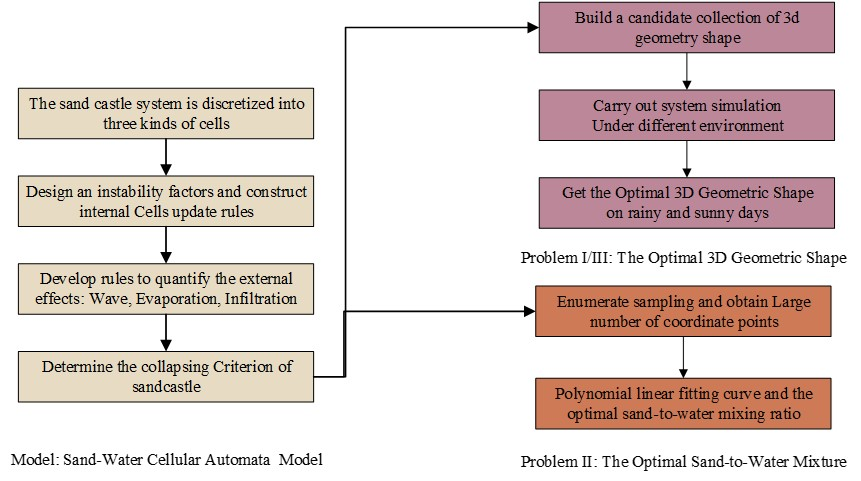
\includegraphics[width=5in]{overview.jpg}
		\caption{Model Overview}
	\end{figure}
	\subsection{Notations}
	Important notations used in this paper are listed in Table \ref{Notations},

	\begin{table}[htbp!]
        \setlength{\belowcaptionskip}{0.2cm}
		\centering
		\caption{Notations}
		\label{Notations}
		\begin{tabular}{clc}
		\hline
			Symbol   & Description     \\ \hline
			$N_{w}^{i}$    & Number of water cells around cell $i$ \\
			$N_{e}^{i}$    & Number of empty cells around cell $i$ \\
			$N_{s}^{i}$    & Number of sand cells around cell $i$ \\
			$T_i$            & Instability factor of sand cell $s_i$ \\
	     	$T_0$            &Boundary instability value for the “fall” of sand cells\\
			$N_{w0}$     & Critical parameter of “dissolution”  \\
			$m$            & Sand-to-water proportion \\
	     	$B$            &Collapsed boundary coefficient\\
	     	$H$         & Height of the sandcastle foundation\\
	     	$k$         & The relative influence of rain on the stability of the 3D geometry
	     	% the height of the bottom of sandcastle foundation 
	     	\\ \hline
		\end{tabular}
	\end{table}
	
    % \section{Model Overview}

	\section{Sand-Water Cellular Automata Model}\label{sec:CA}
% 	基于我们的假设,海滩边的沙堡是可以看做是由沙子、水分、空气三种基本粒子组成的一个系统,系统会受到内外两部分的影响,内部的粒子之间互相存在力的约束作用,当处于某一状态时,沙堡系统保持稳定;外部会受到海浪冲刷、光照蒸发、水分下渗等诸多因素的影响。所以,对于一个像这样的复杂动态系统,我们可以利用元胞自动机来对其进行模拟。形式化来说,元胞自动机是一种将动态复杂系统定义为由离散有限状态的细胞构成的细胞空间的方法,其通过特定的规则,细胞将在离散的时间维度进行更新。所以,元胞自动机是一种模拟沙堡系统的很好的方法。
\subsection{Model Principle}
    According to our assumptions, the sandcastle foundation can be viewed as a system composed of three kinds of basic particles: sand, water, and air. The system is affected by the internal and external factors: the binding force of internal particles will promote the stability of the system, whereas various factors, namely wave erosion, sunlight evaporation, and water infiltration, which will accelerate the collapse of the sandcastle. Therefore, for such a complex dynamic system, cellular automata can be applied for a solution. Formally, cellular automata is a dynamic system defined in a cell space composed of cells with discrete and finite states. According to certain local rules, these cells evolve in discrete time dimensions. Thus, the simulation based on Cellular Automata (CA) is a good approximation to the sandcastle foundation.
	
	\subsection{Description of System Construction}
% 	We physically characterize the system in following aspects:
    The most basic unit of the Cellular Automata is cell. Each cell is described with the following characteristics. 
 	\begin{itemize}
	   % \item Cell is the most basic unit of cellular automata.
	    
	    \item  Cells can memorize storage status.
	  
       \item Each cell of the cellular automata has three states, namely empty cell, water cell, and sand cell.
	    
 	    \item The state of any cell at next moment is determined by its own state and the states of its 26 neighbors, with certain rules, which is demonstrated in Figure~\ref{fig:The Schematic Diagram}.

 	\end{itemize}

	\begin{figure}[htbp!]
		\centering
		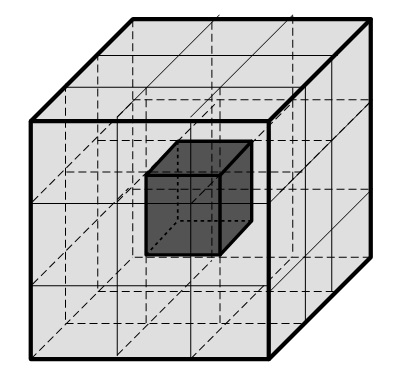
\includegraphics[width=0.25\columnwidth]{The Schematic Diagram.jpg}
		\caption{The Schematic Diagram}
		\label{fig:The Schematic Diagram}
	\end{figure}
	
 	
	\subsection{The Rules}\label{sec:rules}
	Considering the behavior of the sandcastle system exhaustively from both the internal and external parts, the following update rules of CA are purposed.
	\subsubsection{Inside the Sandcastle}
	\begin{enumerate}
	   \item All cells cannot move upward. Each cells can only move to the grid at any given time.
	   \item To quantify the tendency of a sand cell $i$ to move, we define an instability factor $T_i$. Then,
	   \begin{equation}\label{eq:unstability}
       T_{i}=a N_{w}^{i}+b N_{e}^{i}+c N_{s}^{i}
      \end{equation}
    where, $a, b, c$ indicates the weight of the contribution of surrounding cells (water/empty/sand cells) to the instability factor of the center grid $T_{i}$ respectively. Intuitively, the increase in the number of sand cells will also increase the compactness of the center grid, while empty cells promote the sparsity. We can therefore assume that $b>0$ and $c<0$ naturally. Considering the nonlinear relationship of solubility and stability, the sign of $a$ is related to the number of surrounding water $N_w$, which will be discussed more detailedly in the section \ref{section:nw0}.

\item If $T \geq T_0$, the sand cells begin to move following the principle:

\begin{itemize}

    \item Sand cells ca move only downward or horizontally, and move downward with probability $\alpha$ while moving horizontally with probability $(1-\alpha)$.

    \item Sand cells will move to only the surrounding water cells and empty cells, and move to the water cells with probability $\beta$ while moving to the empty cells with probability $(1-\beta)$.

    \item After obtaining the exchange probabilities of the surrounding 26 cells, we use probability sampling to determine the exchange target position of the certain sand cell.

\end{itemize}
 
\item If instability factor $T_i<T_0$ , the sand cell keeps still. 

\item If the number $N_{s}^{i}$ of sand cells around a water cell $i$ satisfies $ N_{s}^{i}>13 $, the water cell holds still. Otherwise, the water cell moves to one of its surrounding empty cells horizontally or downward with certain probability.

\item The sand and empty cells in the sandcastle foundation no longer update their states.

\item The water cell at the foundation will seep into the ground following the principle: 

\begin{itemize}

    \item The water cell at height $h$ will seep into the ground (\ie, turns itself into empty cell) with the probability $P=P_\text{seep} (1-\frac{h}{H})$, which is positively related to its height. 
% In other words,The water cell at height $h$ will become empty with the probability $P=P_{seep} (1-\frac{h}{H})$. 
% Specially,The water cell at height H will seep into the ground with the probability 1.

\end{itemize}
	\end{enumerate}
	\begin{figure}[htbp!]
	    \centering
	    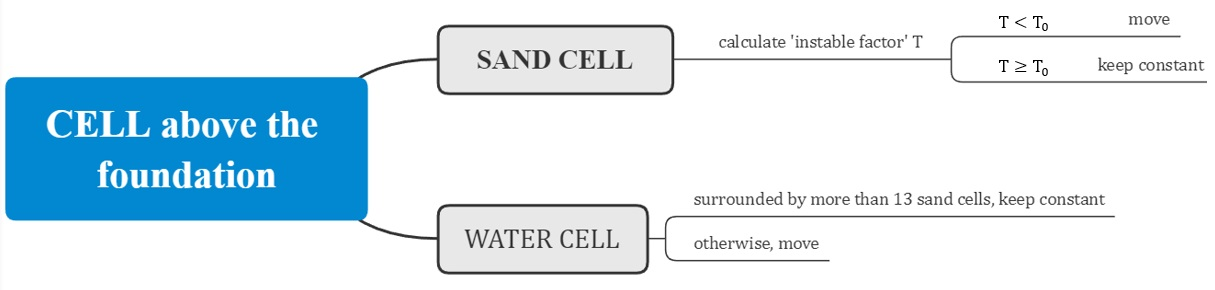
\includegraphics[width=0.8\columnwidth]{Transition Rule of Sand and Water Cell.jpg}
	    \caption{Transition Rule of Sand and Water Cell}
	    \label{fig:Transition Rule of Sand and Water Cell}
	\end{figure}
	
	\subsubsection{The Impact of Waves and Rain}\label{wave and rain}
   \begin{itemize}
   
	 \item \textbf{Wave:} ``Sea waves'' (composed of water cells) appear on the left side of the model with a certain pattern and have effects on only the surface of sandcastle foundation, and the cells on the surface change state following the principle:
     
     \begin{enumerate}
     
    
        \item  If there is an empty cell to the right of "sea wave", this empty cell will convert into a water cell with the probability $P=P_\text{wave}$.
     
         \item If there is a sand cell to the right of ``sea wave'' and its instability factor $T_i \geqslant T_2$, where $T_2$ is the boundary condition of sand movement, we reached the conclusion that $T_{i} \in[26 c, 26 b]$ in Section~\ref{T0anyla}. Therefore, we can use relative instability factor as the probability of converting sand cell to water cell,  \ie  this sand cell will convert into a water cell with the probability $P=\frac{T_i-26c}{26b-26c}$.
     
     \end{enumerate}
     
     \item \textbf{Rain:} The cells on the surface change state following these principles when raining:
	
	\begin{enumerate}
	    \item The empty cell on the surface will convert into a water cell with the probability $P=P_\text{rain}^e$.
    
	    \item The sand cell on the surface will convert into a water cell with the probability $P=P_\text{rain}^s$.
	\end{enumerate}
	
	\end{itemize}

	\subsubsection{Other Impacts}
	\begin{itemize}

	\item \textbf{Evaporation:} Evaporation has effects on the surface of the sandcastle, and the water cell on the surface will convert into an empty cell with the probability $P=P_\text{evap}$.
    
    % 记初始时沙堡地基以上部分的沙细胞个数为 $N_0$,当在
    \item \textbf{Collapse:} Let the number of sand cells above the foundation be $N$ and its initial value $N_0$, sandcastle collapses at $i$-th iteration if $N_i \leq \frac{N_0}{B}$, where B is a collapsing coefficient.
	\end{itemize}

	All cells together form the sand castle system, and we can simulate various phenomena as shown in Diagram~\ref{fig:whole}.
	
		\begin{figure}[thbp!]
		\centering
		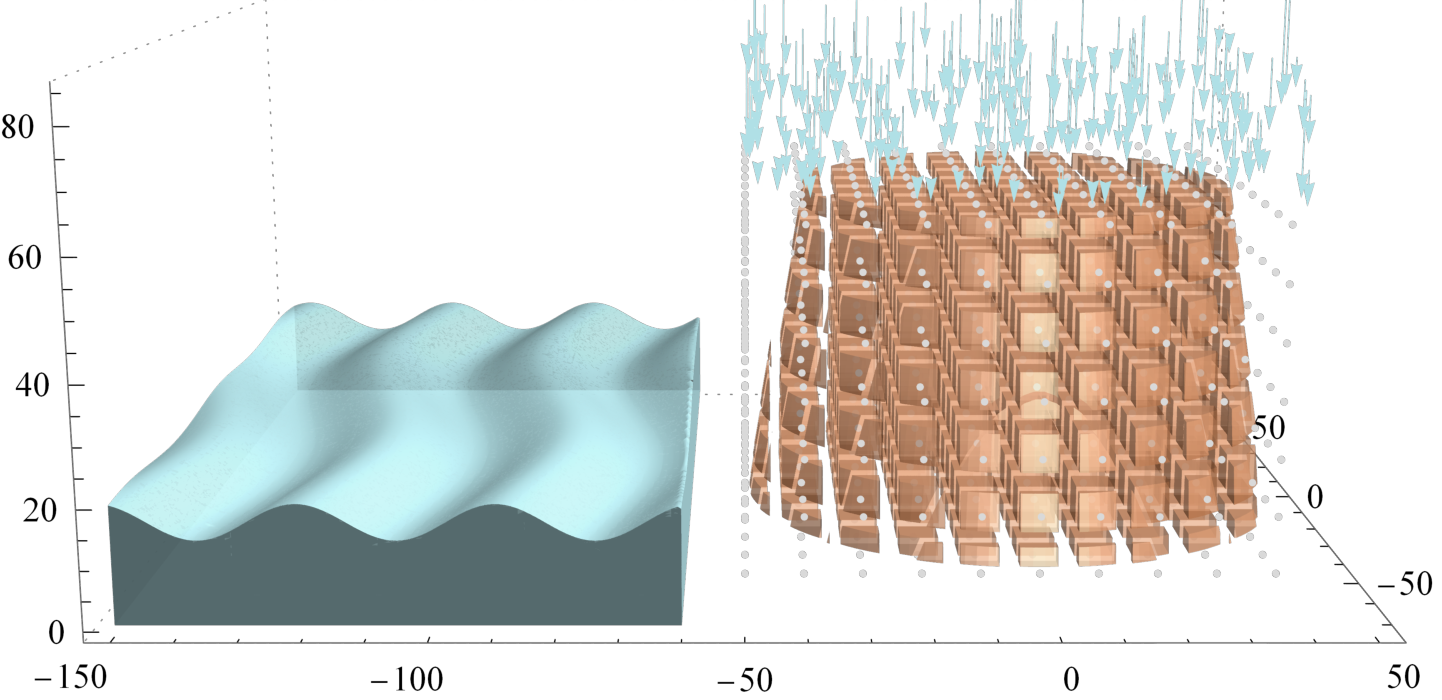
\includegraphics[width=0.75\columnwidth]{brownCell-clearWave-Rain.pdf}
		\caption{Our sandcastle simulation system}
		\label{fig:whole}
	\end{figure}
	
	
	
    \subsection{Parameter Estimation}
	\subsubsection{Estimation of $N_{w0}$}\label{section:nw0}
	To describe the moving trend of the cells inside the sand-water CA, we proposed an instability factor $T$ of a cell in Equation \ref{eq:unstability}, which is a linear function of the number of different cells surrounding. To determine the impact of the number of water cells to instability $a$ accurately, we consider the dissolution as follows:
	\begin{itemize}
	    \item When there is not enough water around a sand cell, \ie~$N_w^{i} < N_{w0}$, the increase in water will increase the dissolution of the sand, thereby enhancing its stability, and thus, $a<0$.
	    \item When there are enough water cells, \ie~$N_w^{i} \geq N_{w0}$, the increase in water will result in the viscous force between water and sand cell, resulting in $a>0$.
	\end{itemize}
	
	Based on the analysis above, we have
	\begin{equation}\label{a sign}
	   \text{sign}(a) =
\begin{cases}
-1 & \text{if } N_w^{i} < N_{w0},\\
+1 & \text{if } N_w^{i} \geq N_{w0}.\\
\end{cases} 
	\end{equation}
    \noindent
    where sign($\cdot$) is a functional symbol; Let $S_v$ denote the maximum volume of sand that water can carry per unit volume, and then we can have an estimate: $N_{w0}=1/S_v$. Following the literature~\cite{hornbaker1997keeps,zhang2020study}, we can set $S_v = 40\%$ and get $N_{w0}=2.5$.

% The sign of $a$ is uncertain, which is related to the number of water cells around cell i. When 	$N_{w}^{i} \leq N_{w}^{0}$, the increase of water cells will promote the dissolution of sand cells and improve the stability, so $a<0$. When $N_{w}^{i} > N_{w}^{0}$, it will make the sand cells become sparse and reduce the instability, so $a>0$.

	\subsubsection{Estimation of $T_0$}\label{T0anyla}
	The instability of sand cell is determined by Equation \ref{eq:unstability}. A sand cell tends to move when its instability $T_i$ is greater than a certain value $T_0$. We can give an estimate of this parameter from a physical perspective:
	
	\begin{itemize}
	    \item \textbf{The most unstable situation}: The sand cells are surrounded by either water cells or empty cells, where we have $T_{\text{max}}=\max(26a,26b)$.
	    \item \textbf{The most stable situation}: The sand cells are surrounded by sand cells, where we have $T_{\text{min}}=26c$.
	\end{itemize}
	
	We define the critical situation between these two extreme situations and have the following approximation of $T_0$:
	\begin{equation}\label{eq:T0}
	    T_0 = \frac{T_{\text{max}} + T_{\text{min}}}{2}
	\end{equation}
	
	Let $|a|=b=c=\frac{1}{\sqrt{3}}$ for convenience, thus $T_0=0$.
	\section{The Optimal 3D Geometric Shape }
	
% 	\subsection{Model Principle}
% 	According to the knowledge of structural mechanics and fluid mechanics, the sandcastle base with a inclined side is the most stable. For a geometric shape, the arris are the most prominent features of the side. Therefore, We choose the most representative shape to do experiment:triangular platform , circular platform and square platform.
	
% 	Many complex problems can be modeled by cellular automata. Cellular automaton is essentially a dynamic system defined in a cell space composed of cells with discrete and finite states. According to certain local rules, these cells evolve in discrete time dimensions. The dynamic system has evolved in the time dimension has been widely applied to various fields of social, economic, military and scientific research.
% 	\subsection{Model Construction}
	
    \subsection{Candidate Geometric Shape}
% 	为了探究沙堡的最佳几何结构体,我们枚举了几种可靠的结构体,在相同的几何参数和环境下,探究能够在我们的塌陷准则下持续最久的最佳几何结构。基于工程机械和实际可行性,我们选择了三种可靠的几何体:圆台、三棱锥、四棱台(见下图)来进行模拟实验。
    To study the best geometric shape of sandcastle, we enumerate several reliable structures. With the same geometric parameter and environment condition, we can explore the best one under our collapsing criterion. Base on engineering machinery and practical feasibility\cite{pakpour2012construct}, we choose 3 types of geometry: circular frustum, triangular frustum and square frustum (see Figure~\ref{fig:3d}).
    
	\begin{figure}[htbp!]
	    \centering
	    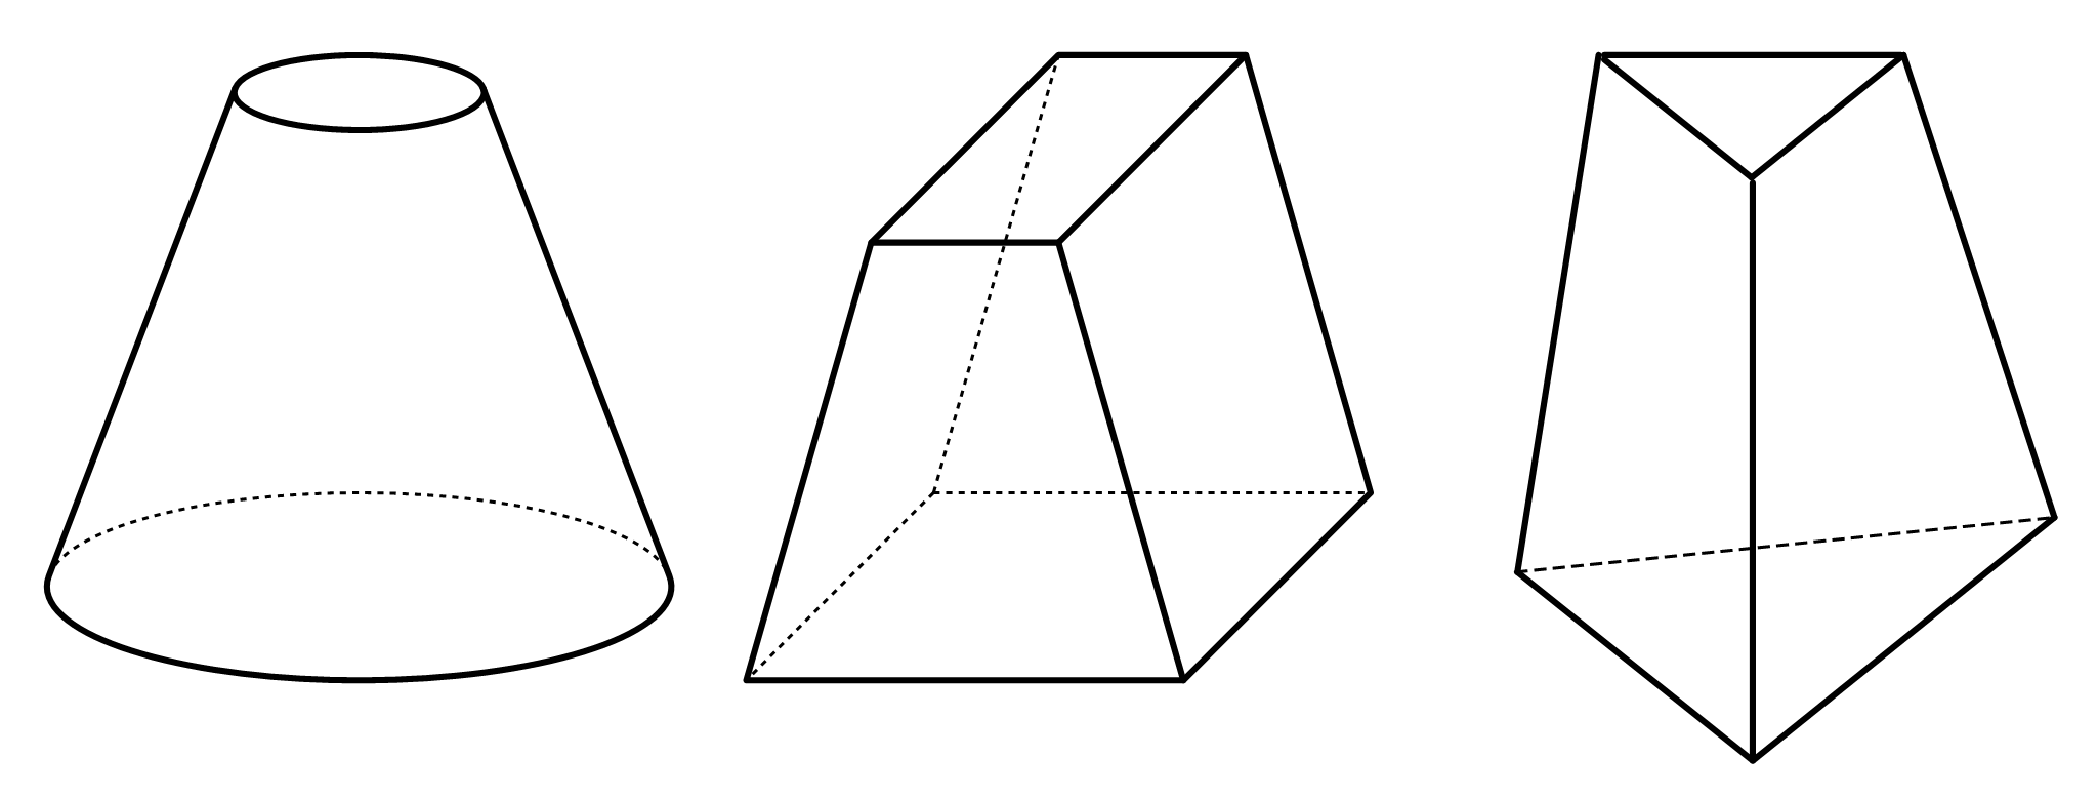
\includegraphics[width=0.6\columnwidth]{3d.pdf}
	    \caption{Geometric Shape to be Tested}
	    \label{fig:3d}
	\end{figure}
    

	\subsection{The Simulation Algorithm}
	Using the sand-water CA model we purposed in Section \ref{sec:CA}, we can evaluate the candidate geometries case by case. The simulation algorithm is shown as follow.
\begin{algorithm}[htbp!]
	\caption{\small{The process of determined optimal 3D geometric shape}}
    	\begin{algorithmic}[1]\small
    		\REQUIRE The sand-water mixing ratio $m$, candidate set $\mathbb{G}$ with $n$ geometry, collapsing coefficient $B$
            \STATE {Initialize CA system for each geometry $G_i$: determine the type of the cells inside the geometry.}
            \FOR{$i{=}1$ to $n$}
            % 得到沙基上部的初始数目N0,初始化轮次t=0
            \STATE get the initial number $N_0$ of the sand cells above the sandcastle foundation, and set $t=0$.
            % 当N/N0 > B时,系统更新
            \WHILE{the number of sand cell above the sandcastle foundation $N \geq B N_0 $}
            % 海浪冲刷,和沙堡表面分子进行作用
            \STATE generate waves composed of water cells and scour the sand castle foundation by applying the "wave" rules motioned in section \ref{wave and rain}.
            % 根据规则,沙堡内部进行分子运动
            \STATE The cells above the foundation exchange internally, and water cells inside the foundation infiltrate with certain probability $P(h)$
            % 阳光照射,沙堡表面水分子以某一概率蒸发
            \STATE The cells on the surface of the sandcastle evaporate with a certain probability.
            % 计算沙基上部新的数目N,t++
            \STATE t++
            \ENDWHILE
            % 得到几何体Gi的塌陷轮次ti
            \STATE Get the collapse iteration number $t_i$ of geometry $Gi$ 
            \ENDFOR
            % 取ti最大的几何体Gi,即为所求
            \STATE The optimal geometry is $G^{*} = \argmax_{G_i} t(G_i)$.
    	\end{algorithmic}
		\label{algorithm1}
\end{algorithm}
	
      	\subsection{Result}
     The result of stimulation is shown in Figure~\ref{fig:Triangular frustum} $\sim$ \ref{fig:Square frustum} and Table \ref{tab:The lasting time of different geometry in sunny day}.
     
            \begin{table}[htbp!]
            	\centering
            	\caption{The lasting time of different geometry in sunny day}
            	\label{tab:The lasting time of different geometry in sunny day}
            	\begin{tabular}{|c|c|c|c|}
            		\hline
            		B &Circular frustum  & Triangular frustum   & Square frustum   \\ \hline
            		2 & 35i & 22i & 29i \\ \hline
            		5 & 68i & 35i & 47i \\ \hline
            		10 & 108i & 67i & 87i \\ \hline
            	\end{tabular}
            \end{table}
            
     
          	\begin{figure}[htbp!]
     		\centering
     		\subfigure[Begin]{
     		\begin{minipage}[t]{0.3\linewidth}%此处的0.3\linewidth控制两张图片之间的距离
     		\centering
     		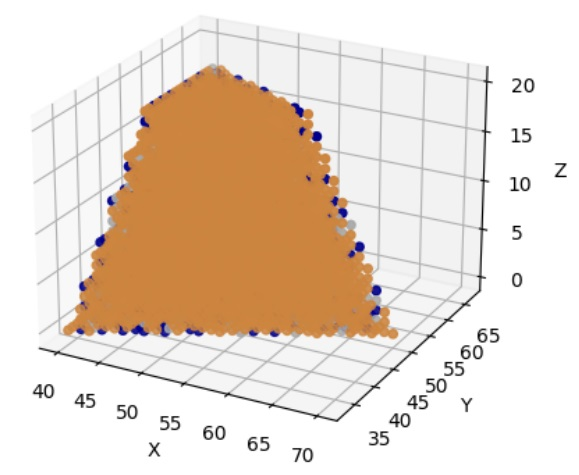
\includegraphics[width=1.8in]{tbegin.jpg}%width控制图片的大小
     		\end{minipage}%
     		}%
     		\subfigure[In the process]{
     		\begin{minipage}[t]{0.3\linewidth}
     		\centering
         	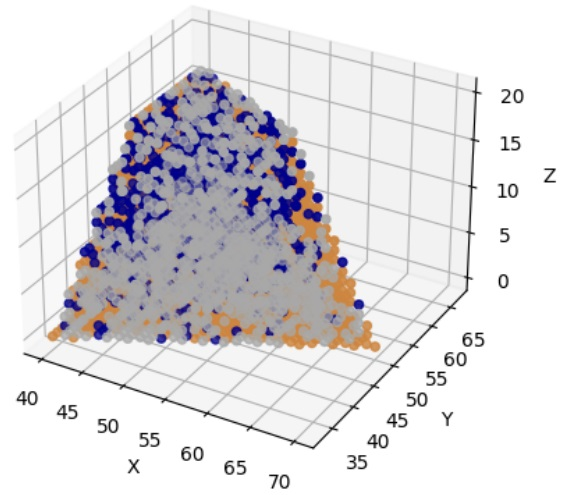
\includegraphics[width=1.8in]{tin.jpg}
         	\end{minipage}%
     		}%
     		\subfigure[End]{
     		\begin{minipage}[t]{0.3\linewidth}%此处的0.3\linewidth控制两张图片之间的距离
     		\centering
     	    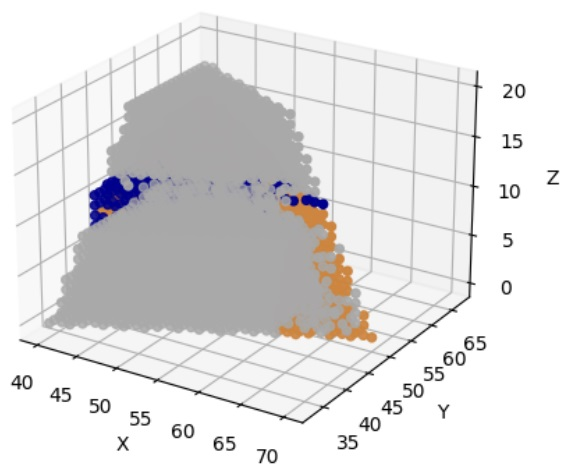
\includegraphics[width=1.8in]{tend.jpg}
     		\end{minipage}%
     	}%
     		\caption{Triangular frustum}\label{fig:Triangular frustum}
     	\end{figure}
     	\newpage
     	    \begin{figure}[htbp!]
     		\centering
     		\subfigure[Begin]{
     		\begin{minipage}[t]{0.3\linewidth}%此处的0.3\linewidth控制两张图片之间的距离
     		\centering
     		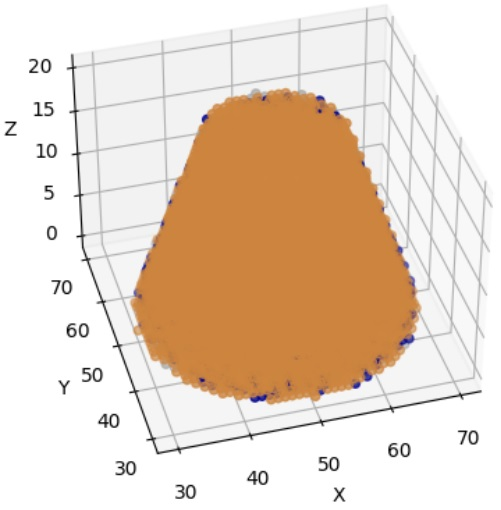
\includegraphics[width=1.8in]{cbegin.jpg}%width控制图片的大小
     		\end{minipage}%
     		}%
     		\subfigure[In the process]{
     		\begin{minipage}[t]{0.3\linewidth}
     		\centering
         	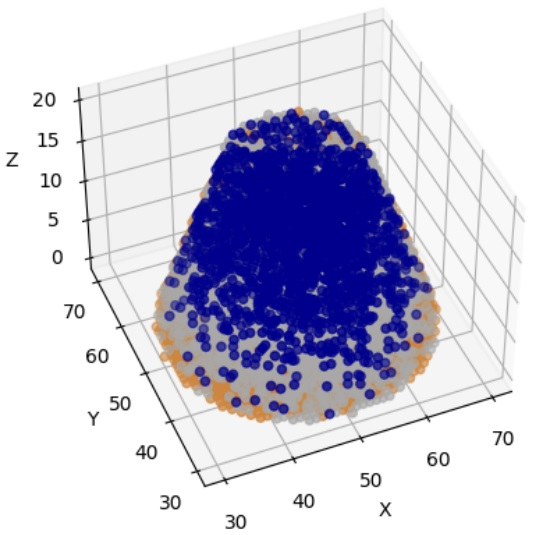
\includegraphics[width=1.8in]{cin.jpg}
         	\end{minipage}%
     		}%
     		\subfigure[End]{
     		\begin{minipage}[t]{0.3\linewidth}%此处的0.3\linewidth控制两张图片之间的距离
     		\centering
     	    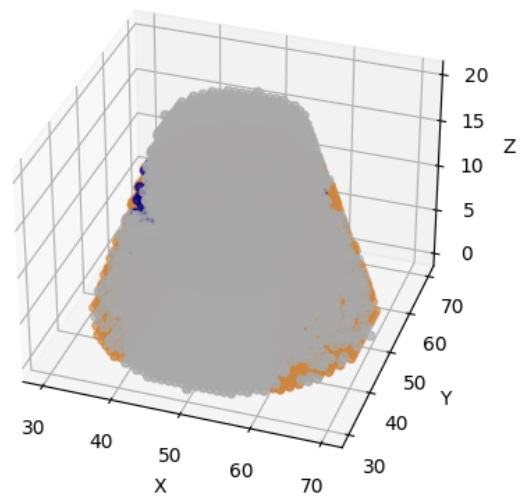
\includegraphics[width=1.8in]{cend.jpg}
     		\end{minipage}%
     	}%
     		\caption{Circular frustum}\label{fig:Circular frustum}%整张图的名称
     	\end{figure}
     	
     	    \begin{figure}[htbp!]
     		\centering
     		\subfigure[Begin]{
     		\begin{minipage}[t]{0.3\linewidth}%此处的0.3\linewidth控制两张图片之间的距离
     		\centering
     		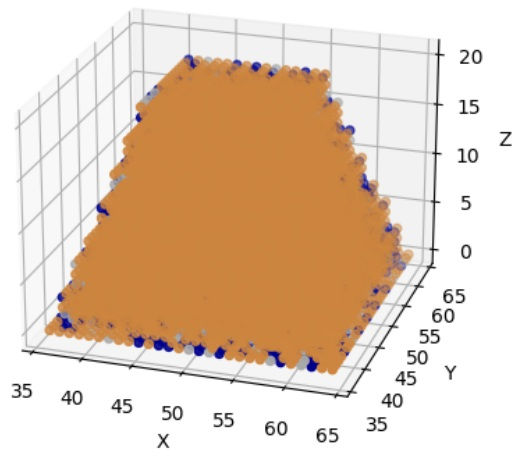
\includegraphics[width=1.8in]{sbegin.jpg}%width控制图片的大小
     		\end{minipage}%
     		}%
     		\subfigure[In the process]{
     		\begin{minipage}[t]{0.3\linewidth}
     		\centering
         	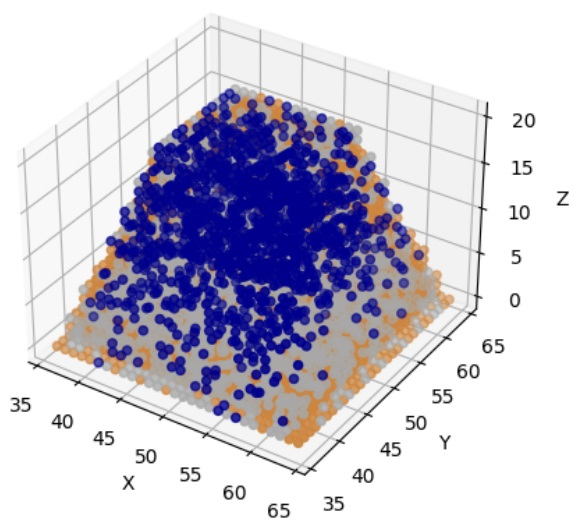
\includegraphics[width=1.8in]{sin.jpg}
         	\end{minipage}%
     		}%
     		\subfigure[End]{
     		\begin{minipage}[t]{0.3\linewidth}%此处的0.3\linewidth控制两张图片之间的距离
     		\centering
     	    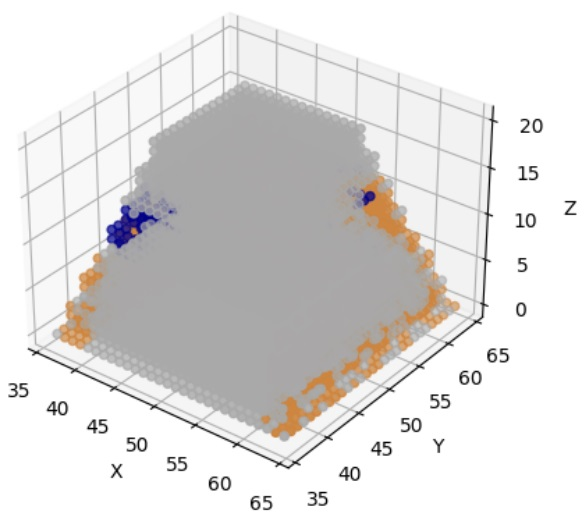
\includegraphics[width=1.8in]{send.jpg}
     		\end{minipage}%
     	}%
     		\caption{Square frustum}\label{fig:Square frustum}%整张图的名称
     	\end{figure}
     
    
     \textbf{Analysis of Result. }
     
     %原型受力均匀,力学,大自然;圆形>正方形>三角形,推出底面越均匀,越对称越稳定,可作为模型推广进一步研究
     From the results of simulation(see Table~\ref{tab:The lasting time of different geometry in sunny day}), it can be seen that the circular frustum lasts longer under the erosion of waves, compared to the others. This result is consistent with our common sense: a round-shaped sandy base is very common on the beach. From perspective of mechanics, the circular structure helps disperse the pressure of the sand castle, thus promote stability.
     Moreover, it can be seen that the collapse time of different 3d geometric shape basically following the rules: circular frustum > square frustum > triangular frustum. Interestingly, the changes of stability seem to related to geometric symmetry, further study can proceed from this phenomenon. 
     
    \section{The Optimal Sand-to-Water Mixture Problem} 
    We do experiment with different water-sand mixture proportion $m_j$. After each experiment, we record the time $(t_j)$ taking to make the sandy base disappear completely, and record the data points $(m_j, t_j)$. By fitting these points, we obtain the best fitting curve. Then we can calculate the optimum proportion of sand-to-water. Our simulation process is summarized with the following pseudo code(see Algorithm~\ref{The process of determined optimal sand-to-water ratio }). 
    \subsection{The Simulation Algorithm} 	
    \begin{algorithm}[htbp!]
	\caption{\small{The process of determined optimal sand-to-water ratio $m$}}
    	\begin{algorithmic}[1]\small
    		\REQUIRE The sample number of sand-water mixing ratio $n_\text{sample}$, sandcastle geometry shape $G$ , collapsing coefficient $B$
    		\FOR {$i{=}1$ to $n_\text{sample}$}
            \STATE {Randomly sample $mi \in [1,+\inf)$ and initialize CA system for geometry $G_i$ by determining all the cells inside the geometry.}
            % 得到沙基上部的初始数目N0,初始化轮次t=0
            \STATE get the initial number $N_0$ of the sand cells above the sandcastle foundation, and set $t=0$.
            % 当N/N0 > B时,系统更新
            \WHILE{the number of sand cell above the sandcastle foundation $N \geq B N_0 $}
            % 海浪冲刷,和沙堡表面分子进行作用
            \STATE generate waves composed of water cells and scour the sand castle foundation by applying the "wave" rules motioned in section \ref{wave and rain}.
            % 根据规则,沙堡内部进行分子运动
            \STATE The cells above the foundation exchange internally, and water cells inside the foundation infiltrate with certain probability $P(h)$
            % 阳光照射,沙堡表面水分子以某一概率蒸发
            \STATE The cells on the surface of the sandcastle evaporate with a certain probability.
            % 计算沙基上部新的数目N,t++
            \STATE t++
            \ENDWHILE
            % 得到几何体Gi的塌陷轮次ti
            \STATE Record the coordinate point ($m_i,t_i$) 
            \ENDFOR
            % 基于前面得到的$n_\text{sample}$个数据点进行9次线性拟合,得到曲线t = F(m)
            \STATE Basing on the previously obtained data points, we can get $t=F(m)$ with 10-degree order linear fitting.
            \STATE The maximum value of curve is the result: $m_{best}=\argmax_m F(m)$
            % 取曲线的最大值对应的m即为最佳混合比
    	\end{algorithmic}
		\label{The process of determined optimal sand-to-water ratio }
\end{algorithm}
    
    
    \subsection{Result}
    \textbf{Sampling and fitting the curve.} Using the optimal 3D geometric shape (\ie~ circular frustum) as sandcastle foundation in our experiment, we adjust the sand-to-water ratio according to the enumeration sampling method. Basing on the Sand-Water Cellular Automata Model, we obtain duration $t$ corresponding to each $m$. Table \ref{tab:Duration of Different Water-sand proportion} is data points generated from our experiment. We assume that the duration $t$ is a function of the sand-to-water ratio $m$. Applying a ten-degree polynomial fitting to these data points, we get the following pictures (see figure~ \ref{fig:Fitting Curve of the circular frustum}).
    \begin{table}[htbp!]
    \centering
	\caption{Duration of Different sand-to-water proportion}
	\label{tab:Duration of Different Water-sand proportion}
    \begin{tabular}{|c|c|c|c|c|c|c|c|c|c|c|c|c|}
    \hline
    sand:water & 1  & 2  & 3  & 4  & 5  & 6  & 7  & 8  & 9  & 10 & 11 & 12 \\ \hline
    duration   & 1 & 4 & 8 & 15 & 18 & 16 & 19 & 18 & 21 & 24 & 22 & 21 \\ \hline
   \end{tabular}
   \end{table}

   \begin{figure}[htbp!]
		\centering
		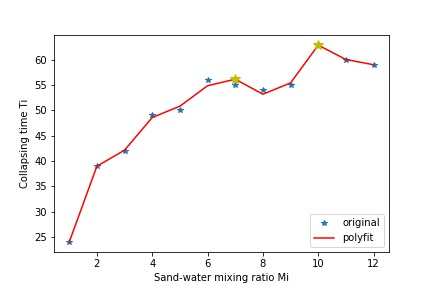
\includegraphics[width=2.5in]{Fitting Curve.jpg}
		\caption{Fitting Curve of the circular  }
		\label{fig:Fitting Curve of the circular frustum}
	\end{figure}

   Similarly, we can acquire the fitting curve of the triangular frustum and the square frustum. The fitting curves are shown in Figure \ref{fig:Fitting Curve}.
   
    \begin{figure}[htbp!]
	\centering
	\subfigure[Triangular frustum]{
		\begin{minipage}[t]{0.4\linewidth}%此处的0.3\linewidth控制两张图片之间的距离
			\centering
			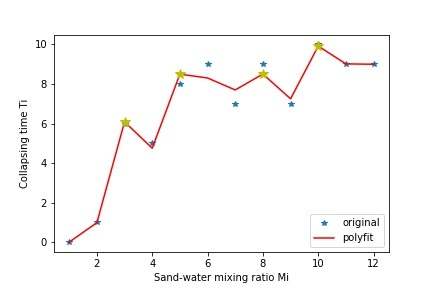
\includegraphics[width=2.5in]{Fitting Curve of T.jpg}%width控制图片的大小
		\end{minipage}%
	}%
	\subfigure[Square frustum]{
		\begin{minipage}[t]{0.4\linewidth}%此处的0.3\linewidth控制两张图片之间的距离
			\centering
			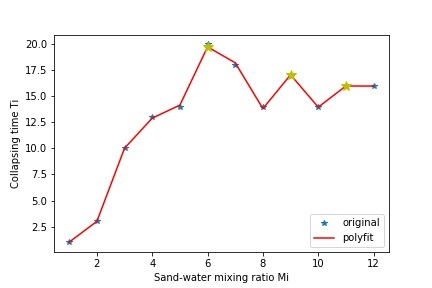
\includegraphics[width=2.5in]{Fitting Curve of S.jpg}
		\end{minipage}%
	}%
	\caption{Fitting Curve}\label{fig:Fitting Curve}%整张图的名称
\end{figure}
   
     \textbf{Analysis of Result.} As can be clearly seen from the Figure \ref{fig:Fitting Curve of the circular frustum}  $\sim$ \ref{fig:Fitting Curve}, for the circular frustum, the  optimal sand-to-water ratio is 10, and in this case, the duration is 25. For the triangular frustum, the optimal sand-to-water ratio is 10 and the corresponding duration is 10. For the triangular frustum, the optimal sand-to-water ratio is 6 and the corresponding duration is 19.
     
     Observe carefully, we can find that sand-to-water ratio has a lot to do with the shape of sandcastle foundation. On the one hand, different 3D geometric shape, the optimal sand-to-water ratio is different. For example, the optimal sand-to-water ratio of circular frustum is 10 while the square frustum is 6. On the other hand, the sand-to-water ratio also influences the optimal 3D geometric shape. From the Figure \ref{fig:Fitting Curve of the circular frustum} and Figure \ref{fig:Fitting Curve}, we can find that the optimal 3D geometric shape is square frustum rather than circular frustum.

    \section{The Optimal Shape in Rainy Day} 	
    \subsection{The Simulation Algorithm} 	
    In this section, we consider the effect of rainfall and set a parameter $I_{\text{rain}}$ to characterize the rainfall intensity. The other parts of simulation are Similar to the previous process.(See algorithm~ \ref{ag:rain})
    \begin{algorithm}[htbp!]
	\caption{\small{The process of determined optimal 3D geometric shape in rainy day}}
    	\begin{algorithmic}[1]\small
    		\REQUIRE The sand-water mixing ratio $m$, candidate set $\mathbb{G}$ with $n$ geometry, collapsing coefficient $B$, rainfall intensity $I_{\text{rain}}$
            \STATE {Initialize CA system for each geometry $G_i$: determine all the cells inside the geometry.}
            \FOR{$i{=}1$ to $n$}
            % 得到沙基上部的初始数目N0,初始化轮次t=0
            \STATE get the initial number $N_0$ of the sand cells above the sandcastle foundation, and set $t=0$.
            % 当N/N0 > B时,系统更新
            \WHILE{the number of sand cell above the sandcastle foundation $N \geq B N_0 $}
            \FOR {$k=1$ to $I_{\text{rain}}$}
            % 下雨冲刷,沙堡的顶面和侧表面细胞在更新规则下更新一轮
            \STATE The top and side surface cells of the sand castle are updated by applying the "rain" rules motioned in section \ref{wave and rain}.
            \ENDFOR 
            % 海浪冲刷,和沙堡表面分子进行作用
            \STATE generate waves composed of water cells and scour the sand castle foundation by applying the "wave" rules motioned in section \ref{wave and rain}.
            % 根据规则,沙堡内部进行分子运动
            \STATE The cells above the foundation exchange internally, and water cells inside the foundation infiltrate with certain probability $P(h)$
            % 阳光照射,沙堡表面水分子以某一概率蒸发
            \STATE The cells on the surface of the sandcastle evaporate with a certain probability.
            % 计算沙基上部新的数目N,t++
            \STATE t++
            \ENDWHILE
            % 得到几何体Gi的塌陷轮次ti
            \STATE Get the collapse iteration number $t_i$ of geometry $Gi$ 
            \ENDFOR
            % 取ti最大的几何体Gi,即为所求
            \STATE The optimal geometry in rainy day is $G^{*} = \argmax_{G_i} t(G_i,I_{\text{rain}})$.
    	\end{algorithmic}\label{ag:rain}
\end{algorithm}

    \subsection{Result}
    % The result of stimulation is shown in Figure \ref{fig:Triangular frustum in rain} $\sim$ Figure \ref{fig:Square frustum in rain}.
    
    
    % \begin{figure}[htbp!]
    % 	\centering
    % 	\subfigure[Begin]{
    % 		\begin{minipage}[t]{0.3\linewidth}%此处的0.3\linewidth控制两张图片之间的距离
    % 			\centering
    % 			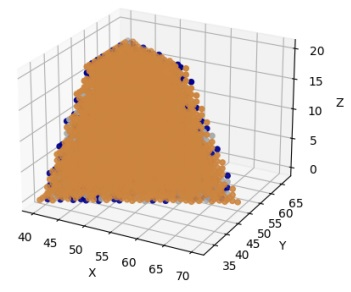
\includegraphics[width=1.8in]{rtbegin.jpg}%width控制图片的大小
    % 		\end{minipage}%
    % 	}%
    % 	\subfigure[In the process]{
    % 		\begin{minipage}[t]{0.3\linewidth}
    % 			\centering
    % 			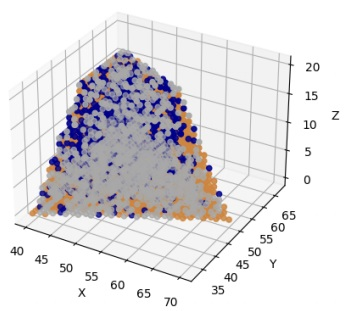
\includegraphics[width=1.8in]{rtin.jpg}
    % 		\end{minipage}%
    % 	}%
    % 	\subfigure[End]{
    % 		\begin{minipage}[t]{0.3\linewidth}%此处的0.3\linewidth控制两张图片之间的距离
    % 			\centering
    % 			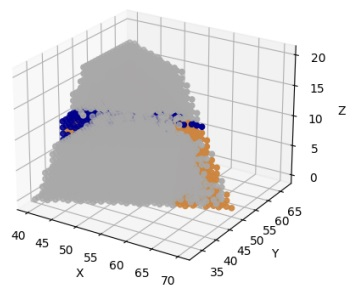
\includegraphics[width=1.8in]{rtend.jpg}
    % 		\end{minipage}%
    % 	}%
    % 	\caption{Triangular frustum }\label{fig:Triangular frustum in rain}%整张图的名称
    % \end{figure}
    % \newpage
    %  \begin{figure}[htbp!]
    % 	\centering
    % 	\subfigure[Begin]{
    % 		\begin{minipage}[t]{0.3\linewidth}%此处的0.3\linewidth控制两张图片之间的距离
    % 			\centering
    % 			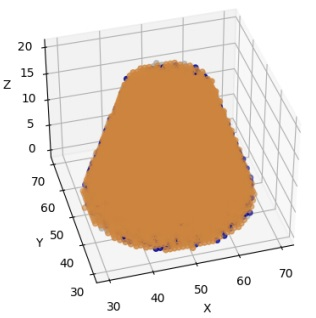
\includegraphics[width=1.8in]{rcbegin.jpg}%width控制图片的大小
    % 		\end{minipage}%
    % 	}%
    % 	\subfigure[In the process]{
    % 		\begin{minipage}[t]{0.3\linewidth}
    % 			\centering
    % 			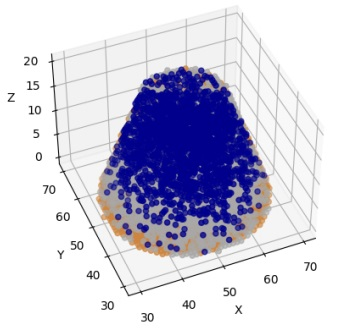
\includegraphics[width=1.8in]{rcin.jpg}
    % 		\end{minipage}%
    % 	}%
    % 	\subfigure[End]{
    % 		\begin{minipage}[t]{0.3\linewidth}%此处的0.3\linewidth控制两张图片之间的距离
    % 			\centering
    % 			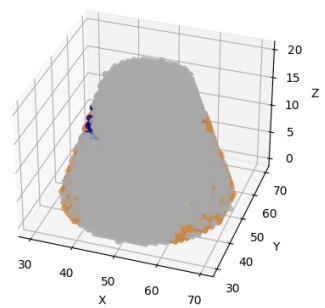
\includegraphics[width=1.8in]{rcend.jpg}
    % 		\end{minipage}%
    % 	}%
    % 	\caption{Circular Platform}\label{fig:Circular Platform in rain}%整张图的名称
    % \end{figure}
    
    %      \begin{figure}[htbp!]
    % 	\centering
    % 	\subfigure[Begin]{
    % 		\begin{minipage}[t]{0.3\linewidth}%此处的0.3\linewidth控制两张图片之间的距离
    % 			\centering
    % 			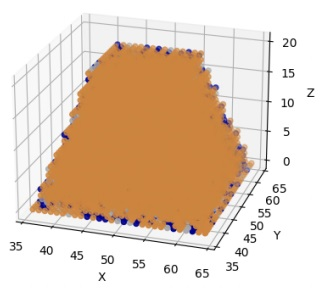
\includegraphics[width=1.8in]{rsbegin.jpg}%width控制图片的大小
    % 		\end{minipage}%
    % 	}%
    % 	\subfigure[In the process]{
    % 		\begin{minipage}[t]{0.3\linewidth}
    % 			\centering
    % 			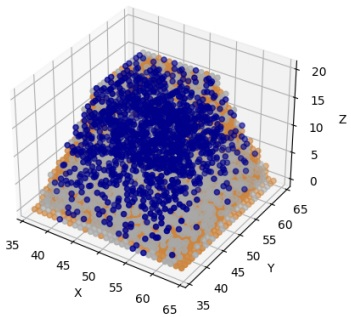
\includegraphics[width=1.8in]{rsin.jpg}
    % 		\end{minipage}%
    % 	}%
    % 	\subfigure[End]{
    % 		\begin{minipage}[t]{0.3\linewidth}%此处的0.3\linewidth控制两张图片之间的距离
    % 			\centering
    % 			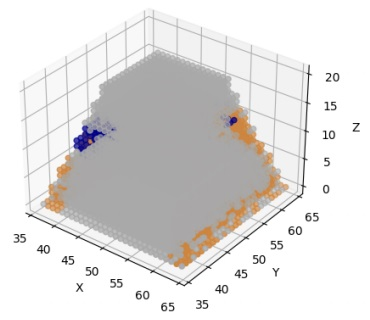
\includegraphics[width=1.8in]{rsend.jpg}
    % 		\end{minipage}%
    % 	}%
    % 	\caption{Square Platform}\label{fig:Square Platform in rain}%整张图的名称
    % \end{figure}
    
    
    
     \textbf{The impact of rainfall intensity. }To explore the impact of rainfall on the sandcastle, we conducted experiments on the circular frustum. By adjusting the rainfall intensity, we get the following results of the first 10 iterations of CA system(see table~\ref{tab:Duration of different geometries under different rainfall intensities}). It can be seen that as the increases of rainfall intensity will accelerate the collapse of sandcastle. 
    \begin{figure}[htbp!]
        \centering
        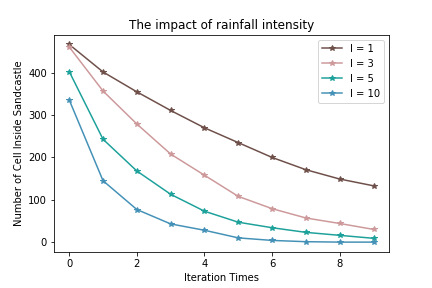
\includegraphics[width=4in]{The impact of rainfall intensity.png}
        \caption{The impact of rainfall}
        \label{fig:the impact of rainfall}
    \end{figure}
    
    \textbf{The optimal 3d geometric shape in rainy day. }We are curious whether the optimal geometric shape remain the same in a rainy environment. With the same parameter setting, we get the lasting time of different 3d geometric shape in rainy day. 
    \begin{table}[htbp!]
    \centering
	\caption{The lasting time of different geometries with different rainfall intensities}
	\label{tab:Duration of different geometries under different rainfall intensities}
    \begin{tabular}{|c|c|c|c|}
    \hline
    $I_{\text{rain}}$ & Circular frustum  & Triangular frustum   & Square frustum   \\ \hline
    1 & 35 & 22 & 29 \\ \hline
    2 & 26 & 17 & 25 \\ \hline
    5 & 21 & 14 & 20 \\ \hline
   \end{tabular}
   \end{table}
 
    From the results, we can see that when there is rainfall, the optimal 3D geometric shape is still circular frustum. 
    
    \textbf{The relative rainfall influence factor $k$. }
    
    Further analysis, we define $k$ as the relative influence of rain on the stability of the 3D geometry as follow. For different 3d geometry shape, we seek to study the difference between their $k$, which show their respective sensitivity to rainfall. 
    \begin{equation}
    	k=\frac{t_{sun}-t_{rain}}{t_{sun}}
    \end{equation} 
    
    In order to study the impact of rain on $k$, we take $B=2,5,10$ for experiment respectively. The results are shown in Figure~\ref{fig:The influence of rain on different geometry}.
 
    \begin{figure}[htbp!]
	\centering
	\subfigure[B=2]{
		\begin{minipage}[t]{0.32\linewidth}%
			\centering
			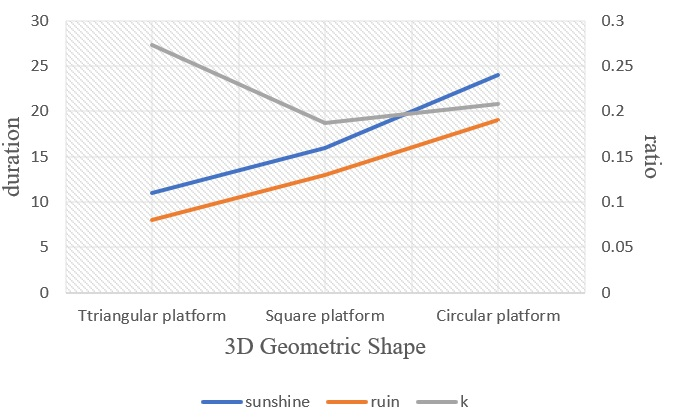
\includegraphics[width=2.3in,height=0.8\linewidth]{B=2.jpg}%
		\end{minipage}%
	}%
	\subfigure[B=5]{
		\begin{minipage}[t]{0.32\linewidth}
			\centering
			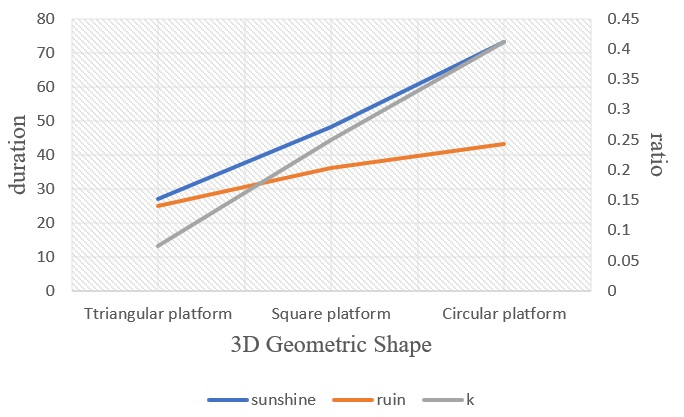
\includegraphics[width=2.3in,height=0.8\linewidth]{B=5.jpg}
		\end{minipage}%
	}%
	\subfigure[B=10]{
		\begin{minipage}[t]{0.32\linewidth}
			\centering
			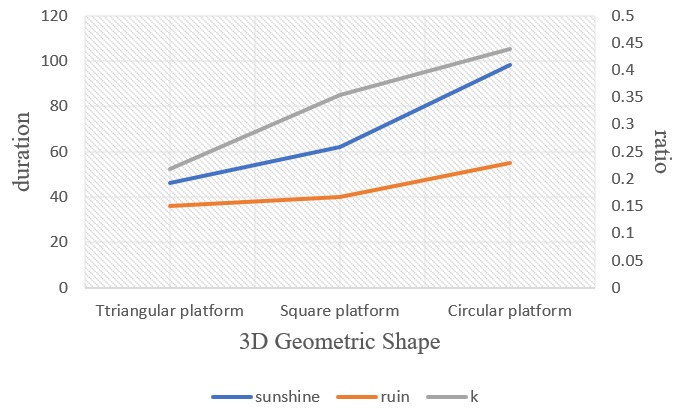
\includegraphics[width=2.3in,height=0.8\linewidth]{B=10.jpg}
		\end{minipage}%
	}%
	\caption{The influence of rain on different geometry }\label{fig:The influence of rain on different geometry}
\end{figure}

    From the Figure~\ref{fig:The influence of rain on different geometry}
	, we can find that the $k$ of the three geometries basically follow the rule: Triangular frustum < Square frustum < Circular frustum. From the perspective of geometry and mechanics, we known that the area of the circle is the largest compared to other 2D geometry(\eg~square and triangle) with the same radius. Since most of the rain falls on the top surface, the rain has the greatest impact on the circular frustum, whose top surface area is the largest. Therefore, it is reasonable that the $k$ of the circular frustum is better than the others.
	

	\section{Test the Model}
	\subsection{Sensitivity Analysis}
	In Section~\ref{sec:rules}, two probability parameters are introduced to characterize the impact of sunlight and rainfall on the sandcastle: rain intensity $I_{\text{rain}}$, and sunlight evaporation factor $P_{\text{evap}}$. The relationship between the lasting time $t$ of sandcastle and these two factors is approximated by the first-order difference,
	\begin{equation}
	\begin{split}
	\frac{\partial t}{\partial I_{\text{rain}}} &\approx \frac{t(I_{\text{rain}}+\Delta I_{\text{rain}})-t(I_{\text{rain}})}{\Delta I_{\text{rain}}}\\
	\frac{\partial t}{\partial P_{\text{evap}}} &\approx \frac{t(P_{\text{evap}}+\Delta P_{\text{evap}})-t(P_{\text{evap}})}{\Delta P_{\text{evap}}}
	\end{split}
	\end{equation}
	
	Therefore, the calculation results are shown in Figure~\ref{sensitivity}.
	
	\begin{figure}[htbp!]
		\centering
		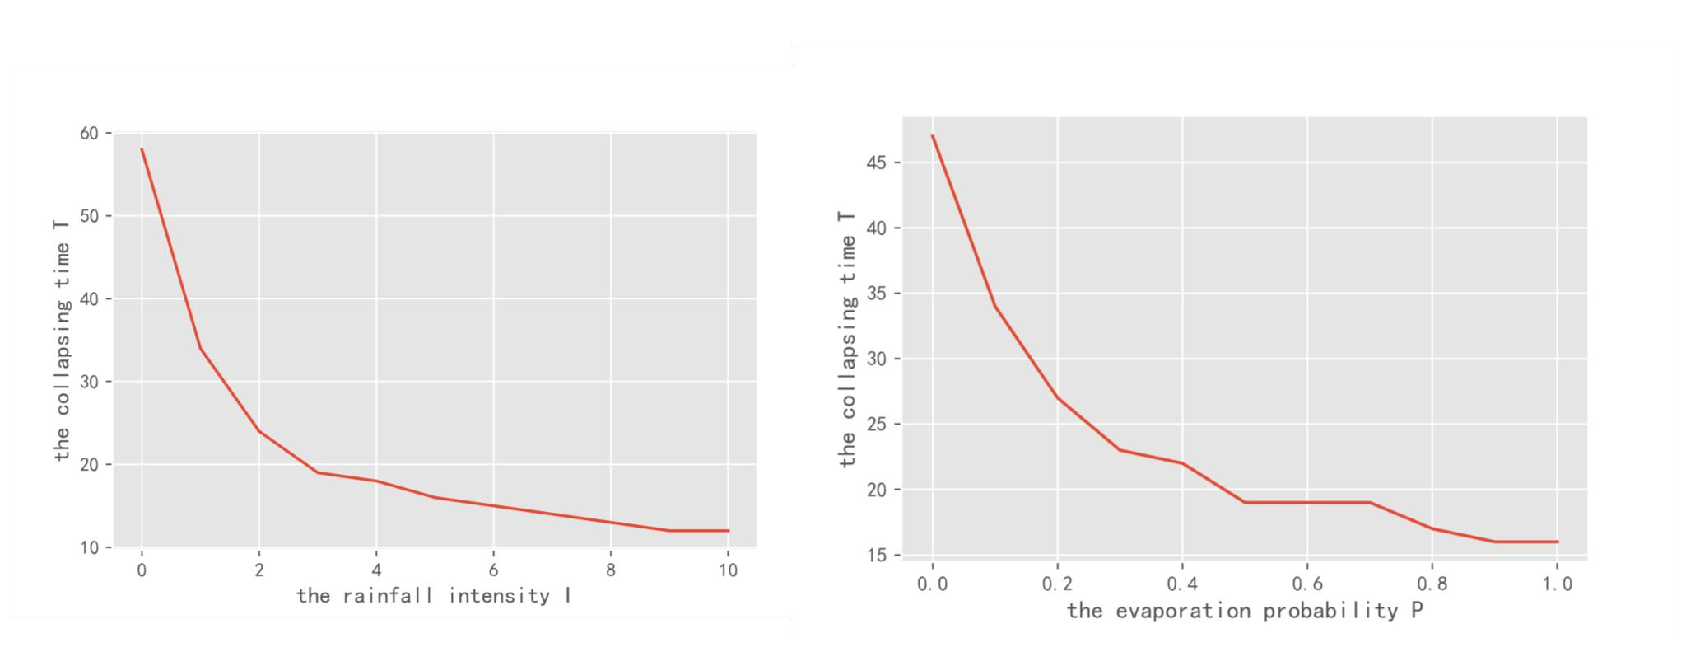
\includegraphics[width=6in]{sensitiy.pdf}
		\caption{Sensitivity analysis of $P_{\text{evap}}$ and $I_{\text{rain}}$}
		\label{sensitivity}
	\end{figure}
	
	It is indicated that the lasting time of sandcastle decreasing along with the rainfall intensity, which reflects the destructive effect of rain on sandcastle; Correspondingly, the lasting time of sandcastle foundation is also decreased with the sunlight evaporation probability, which shows that sunlight will accelerate the collapse of sandcastle. The trend of the model obtained by sensitivity test is consistent with the actual situation, which also proves the rationality and robustness of our CA model of sandcastle foundation.
	
	\subsection{Robustness Analysis}
	Through the above analysis, we obtained the optimal shape of the sand base and the optimal sand-water ratio. Meanwhile, we presume many parameters in the model. In order to ensure the robustness of the model, we test the model from the following aspects.
	%(Due to time constraints, 
	Analysis is performed on only the cone frustum, which is similar to other geometric shapes.
	
	\begin{itemize}
	    \item \textbf{Collapsing coefficient $B$}: The critical condition of the upper surface being destroyed. Since the castle is to be built on the mound, it is important to have a stable one. In the above experiment, when $N_t < \frac{N_{0}}{B}$, it is considered that the surface of the sand base has been damaged, and it is not qualified for building a castle, so $N_\text{min} = \frac{N_{0}}{B}$. When we change the value of $B$, the best sandcastle model may change.
	    \item \textbf{Critical instability $T_0$ of sand cells}: In the simulation process, by considering two extreme physical situations, we have an estimate that the critical stability factor for a sands cell to move is $T_0$. Thereby, it is judged whether or not the sand will move based on $T_0 = 0$.
        Depending on the critical value, the movement of the sand cell is different. Then, the stable state of the sand base may also change.
         \item \textbf{The width of the sand base $L$}: According to common sense, items with a large foundation area stand more stable than those with a small foundation area. For sandy foundations, a larger sandy foundation facilitates the dispersion of the wave impact and also therefore a longer duration of life. The choice of this parameter may have an impact on the choice of the optimal sandcastle model.
        

	\end{itemize}
	
	 Our model design allows us to change these parameters. Next we will analyze in detail the effect of the following elements on the model:
        \begin{enumerate}
            \item Sand Foundation Damage Judgment
            \item Unstable Factors
            \item Geometric Shape’s Length Attribute
        \end{enumerate}
	We record the results in each case with changes of -10\% and +10\%. The results are shown in Table ~\ref{tab:robusness table}, where $i$ denotes the round of iterations.
	
	
	\begin{table}[hbtp]
		\centering
		\caption{Results of Robustness Analysis}
		\setlength{\tabcolsep}{10mm}{
			\begin{tabular}{cccc}
				\hline
				~            & -10\%     & 0   & +10\% \\ \hline
				$B$ & 34$i$ &60$i$ &  71$i$     \\
				$T_0$  & 43$i$  &60$i$ & 65$i$ \\
				$ L $ & 58$i$ &60$i$  &64$i$ \\\hline	\end{tabular}\label{tab:robusness table}
		}
	\end{table}
	
	Based on the above data, we can see the range of influence of these parameters on stability.
% 	The analysis results of the  analysis indicate that the effect of the sediment capacity on the sand foundation cannot be underestimated. To build a stable sand foundation, choosing the appropriate sand is essential. We should try to find sand with strong adhesion, so as to relatively reduce the ability of the waves’ sediment.
	
    From the results of the analysis of the geometric properties of the sandcastle, the establishment of a wider sand base is also a feasible way to improve its stability. The wider the sand base is, the easier it is to disperse the wave impact on it, thus making the life span longer.
    
    % The analysis results of instability factors show that the adhesion between sand and water also has a huge impact on the stability of sand foundation.
    The analysis of the critical condition $T_0$ shows that it affects the stability of the internal structure of the sandcastle, which is reflected in the duration of the sandcastle. When the value of $T_0$ is relatively large, the cells inside the sandcastle have a tendency to remain stationary, so the sandcastle becomes relatively stable; conversely, when the value of $T_0$ is relatively small, the sandcastle is more likely to collapse because the internal cells have a strong tendency to move.
    % Nevertheless, we get the same result under each condition.
    
    The results of the sensitivity analysis of the sandcastle damage judgement showed that whatever was used as the basis for the judgement did not affect the final results of the model.

	It can be seen that the duration of the sandcastle remains essentially constant despite the change in the parameter set, which verifies the robustness of our model.
% 	It means that the similar final fish distribution can be obtained on the premise of different initial fish distribution, which verifies the decisive role of temperature change on fish migration and reflects the stability of the model.
% 	\newpage
	\section{Strategies to Make sandcastle More Lasting}
	Based on the results of the sensitivity analysis and our discussions, we find out the strategies below to increase the stability of the sandy foundation.
	\begin{itemize}
	    \item \textbf{Try to keep the sand castle away from the sea.} As the primary external factor that erodes the sand castle, waves usually reach the strongest effect at the seaside, and as the distance increases, the impact of its erosion will gradually weaken. Therefore, it is best to arrange sand castles far away from the sea to achieve the longest duration. 
	    \item \textbf{Replace some plastic boards around the sand castle to prevent the impact of precipitation.} As one of the natural "enemies" of the sand castle, heavy rainfall will disintegrate it from the upper surface of the sand castle. In order to cope with this situation, if possible, it would be good to build some waterproof facilities around the sand castle. 
	    \item \textbf{Protect sand castle from strong evaporation effect.} In the summer, it is usually accompanied by high temperature and strong sunlight. At this time, the water on the sandcastle evaporates since continuously exposure to sunlight. The sand castle become dried and the viscosity of the water and sand inside is insufficient to support itself, thus become unstable. Similarly, it would be nice to some facility(\eg~Parasol) around the sand base.
	\end{itemize}
	\section{Strength and Weakness}
	\subsection{Strength}
    \begin{itemize}
        \item The sensitivity analysis of the model demonstrates the effectiveness of the model under different parameter combinations and prove the robustness of the model.
        \item We carry out reasonable simplification, and establish a cellular automaton model to solve the problem. The results are consistent with actual practice, and have high credibility.
        \item In addition to the sea and rain erosion mentioned in the problem description, various external effects that the sand castle may encounter are considered,\eg~,evaporation, water infiltration. This makes our model more convincing and close to the actual situation.
        
    \end{itemize}
    
	\subsection{Weakness}
	\begin{itemize}
	    \item Some assumptions of cell update rules are too idealistic, which may lead to the situation contrary to the actual in extreme cases. 
	   %\item Lack of solid theoretical foundation while modeling the internal pattern of sandcastle foundation.
	    \item Limited to the limitation of equipment, the cellular automaton model is not quite exact, and the quality may not meet our higher expectations.
	    
	   
	\end{itemize}
    
% \addcontentsline{toc}{section}{Article} 
\addcontentsline{toc}{section}{References and Appendices}
\bibliography{ref}

\section*{Appendices}
% \addcontentsline{toc}{section}{Appendices}
\subsection*{Appendix A Tools and software}
%\addcontentsline{toc}{subsection}{Appendix A Tools and software}
Paper written and generated via \LaTeX, free distribution.\\\indent Graph generated and calculation using Python and MATLAB R2020a.
\subsection*{Appendix B The Codes}
Here are simulation programmes we used in our model as follow.
% \newpage % 应该不用换页? --gjx
\lstinputlisting[language=Python,breaklines=true]{./code/code.py}
\end{document}